
% \chapter{Background}
% \label{ch:Background}

% {\bf ARM TrustZone}~\cite{trustzone} is a widely available hardware-based TEE
% (Trusted Execution Environment) that partitions a device's CPU, memory, and
% peripherals, into two isolated logical ``worlds'' --- normal and secure. Each
% CPU core runs either in a non-secure state, where it has access only to
% resources assigned to the normal world, or a secure state where it has access to
% both normal and secure world resources. When switching between states (e.g., via
% the {\tt smc} instruction), the secure monitor, a critical and heavily-vetted
% software, is invoked to safely perform the transition. TrustZone enables a
% trusted OS to run in the secure world in conjunction with an OS in the normal
% world, and it protects state in the secure world even if the normal world is
% compromised.

% {\bf OP-TEE}~\cite{optee} is an open-source software stack that facilitates the
% use of ARM TrustZone. It provides a secure world OS (OP-TEE OS) for executing
% trusted applications; a low-level secure monitor for switching a core between
% non-secure and secure states; a TrustZone driver for normal world OSes such as
% Linux, which enables regular user-space applications to execute RPCs in the TEE;
% and a user-space supplicant that enables applications running in the TEE to
% access resources in the normal world OS.

\chapter{TrustZone \& OP-TEE Overview}
\label{ch:trustzone}

Trusted capsules allow advisory policies to be enforced on remote devices that the data owner does not
control. To protect sensitive operations such as trusted capsule policy evaluation
from remote users who can run an arbitrarily software stack, we require a Trusted Execution Environment (TEE) that is resistant to potential compromise of both applications and OS running on the remote device. 
We use
%Our trusted capsule data monitor uses 
\textbf{ARM TrustZone} technology as our hardware-based \textbf{Trusted Execution Environment} 
%to provide such a hardware-based trusted 
%execution environment (TEE)  
and \textbf{Linaro OP-TEE} as the operating system that runs in our TEE.
%TrustZone software stack. 
Within this TEE, we handle sensitive cryptographic operations, perform policy evaluation, 
securely store policy state, and establish a secure channel to the remote policy coordinator server. 

In the following, we provide a brief overview of the properties of TrustZone and OP-TEE. 

\section{TrustZone}

\textbf{ARM TrustZone}~\cite{trustzone} %provides a hardware-based TEE. It 
is widely available on current commodity ARM processors. A TrustZone enabled processor maps to two virtual processors that that execute in a time-sliced fashion,context switching between each other through a special core mode called the \say{monitor mode}. We call a virtual processor that is running in the TEE to be running in \textbf{Secure World}. A virtual processor that runs the regular operating system is said to be running in \textbf{Normal World}. The monitor mode software acts as a robust gatekeeper to manage the physical processor's context switch between these virtual processor modes by means of interrupt handling. These modes of operation of a physical processor and the transitions between them are visualized in Figure ~\ref{fig:SMC_transition}.

\begin{figure}[h]
\centering
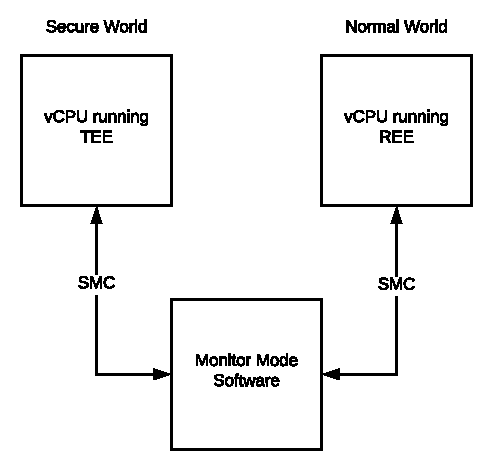
\includegraphics{fig/SMC_SW_NW.pdf}
  \caption{The Physical CPU maps to two virtual CPUs - one running the TEE (secure world) and the other running the rich OS (normal world). The context transitions between these are handled by the \texttt{smc} instruction that gets serviced by the monitor mode software, which runs at the highest level of privilege. }
    \label{fig:SMC_transition}
\end{figure}

% The mechanisms by which the physical processor running in normal world can enter the monitor mode for context switching is tightly controlled and are treated as exceptions by the monitor mode software. 

One way in which world switch can be triggered by the software is by executing a dedicated instruction, the Secure Monitor Call (SMC) instruction. The software that runs in the monitor mode is defined by the implementation of the chipset, but it generally saves the state of the current world and restores the state of the world being switched to. Once the restoration is complete, the monitor performs a return-from-exception call to restart the processing in the restored world.  

A TrustZone enabled processor implements three sets of interrupt vectors - one for each world, and one for the monitor mode. The locations of these tables are programmable and can be modified by changing the appropriate Vector Base Address Register. This can be used to control where the \textit{smc} instruction will trap to. 

The ARM TrustZone security model provides the following hardware-based guarantee: 
\textbf{the normal world cannot access the registers, memory or peripherals assigned 
to the secure world; but the secure world can access normal world registers and memory}.\footnote{TEEs cross-world ability to manipulate the memory and registers are grounds for Spectre\cite{Kocher2018spectre} and Meltdown\cite{Lipp2018meltdown} type bugs. This has been acknowledged by Linaro and ARM and they have published page table isolation patches to fix these\cite{bech_biesheuvel_brown_thompson_2018}.} 

This security guarantee for register access is maintained by tracking the execution mode of a processor. The monitor mode software executes in secure world. The world in which a processor is currently executing is indicated by the NS-bit in the Secure Configuration Register (SCR) in the system control coprocessor (CP15). When in monitor mode the processor is running in Secure World, regardless of the value of the NS-bit, but operations on the banked CP-15 registers will access the Normal World copies if the SCR NS-bit is set to 1. 

For memory, the secure world provides such a guarantee by either taking exclusive control of on-chip 
memory such as secure SRAM~\cite{hikey} or by mapping a section of the general off-chip memory and hiding it 
from the MMU of the normal world.

For peripherals, secure and normal world access are partitioned by interrupt modes. 
ARM processors contain two interrupt modes -- FIQ (Fast Interrupt Request) and IRQ (Interrupt Request). Each interrupt mode can be individually assigned to trap to code in the normal or secure world. Therefore, a peripheral can be assigned to a specific world by assigning it to the corresponding interrupt mode. The usual set-up 
assigns FIQ to the secure world and IRQ to the normal world, as most existing normal world drivers 
currently operate using the IRQ mode.

For additional hardware protection for off-chip memory and device protection, additional hardware, 
such as TrustZone Protection Controller (TZPC) and TrustZone Address Space Controller (TZASC), can
be added to extend the dual-world abstraction to the AXI-bus, memory controllers and interrupt controllers. This is done by propagating the NS-bit over the system bus. 


% Please add the following required packages to your document preamble:
% \usepackage{graphicx}
\begin{table}[]
\centering
\resizebox{\textwidth}{!}{%
\begin{tabular}{|l|c|c|}
\hline
\makebox{\textbf{Exception Level}} & \makebox{\textbf{Secure World}} & \makebox{\textbf{Normal World}} \\ \hline
EL0 & Trusted Application & Application \\ \hline
EL1 & Secure OS & Normal OS \\ \hline
EL2 & -         & Hypervisor \\ \hline
EL3 & \multicolumn{2}{c|}{Secure Monitor} \\ \hline
\end{tabular}%
}
\caption{The privilege levels at which the various components of the TrustZone based system run. The Secure Monitor runs at the highest privilege.}
\label{tab:privilege_levels}
\end{table}

The secure monitor operates at Exception Level(EL) 3 - a higher privilege level than both the application (trusted or regular) and the operating system (secure or normal). The Secure OS and the Normal OS operate at EL1, while the Applications - both in secure and normal world - run at EL0. This is shown in Table ~\ref{tab:privilege_levels}.

%It's security capabilities are similar to two 
%separate physical machines connected by a thin communication interface, but packaged more compactly as a 
%single-chip solution. 
%Alternatively, TrustZone can be replicated architecturally with two CPUs, 
%TrustZone's world abstraction has the advantages of requiring less on-chip space, 
%being more energy efficient and enabling symmetric processing. 

\section{Linaro OP-TEE}

\textbf{Linaro OP-TEE} is an open-source operating system that has been designed for ARM
TrustZone. Linaro is part of the industry consortium called Global Platform, which leads efforts in standardizing APIs exposed by different TEE OS vendors. OP-TEE is the OS and related firmware that incorporates this standardized API and is ported across several hardware vendors. 

OP-TEE is the secure OS for executing trusted applications and is composed of:
\begin{enumerate}
    \item A low-level secure monitor for world-switching (ARM Trusted Firmware). This is where the SMC implementation resides.
    \item A TrustZone driver (OP-TEE Linux driver) which is used to access the TEE services from the normal world, and
    \item OP-TEE Supplicant which runs in normal world user space as a single threaded application and is responsible for accessing services expected by the TEE-OS. 
\end{enumerate}

The remaining discussion in this section is based arouind the HiKey system-on-chip (SoC) with Debian Linux as the normal world OS. This is configuration we used for this project. 

\subsection{ARM Trusted Firmware}
\textbf{ARM Trusted Firmware (ATF)}~\cite{atf} provides a reference implementation of the Secure Monitor and the varoius Arm interface standards around system control and management, secure boot conventions, and interrupt management interface. It is the critical piece in booting the secure environment, a process which is outlined in Figure ~\ref{fig:bootsequence}. There are three bootloaders involved in the process, and each is responsible for initializing the image for the next level in the process. BL2 loads all images in the third level of initialization. A root-of-trust can be built by having each stage attest the image of the next. 

%In ATF, transition between boot stages is controlled by several key global data structures:

%\begin{itemize}
%\item  \textit{entry\_point\_info} -- controls the privilege level of the CPU after executing 
%\textit{eret} or \textit{smc}
%\item  \textit{image\_info } -- image size of each boot stage
%\item  \textit{mem\_info\_t} -- available secure SRAM
%\item  \textit{bl31\_params} -- stores information about the secure and normal world OS images 
%for the secure monitor
%\end{itemize}

%%%%%%%%%%%%%%%%%%%%
\begin{figure}
\centering
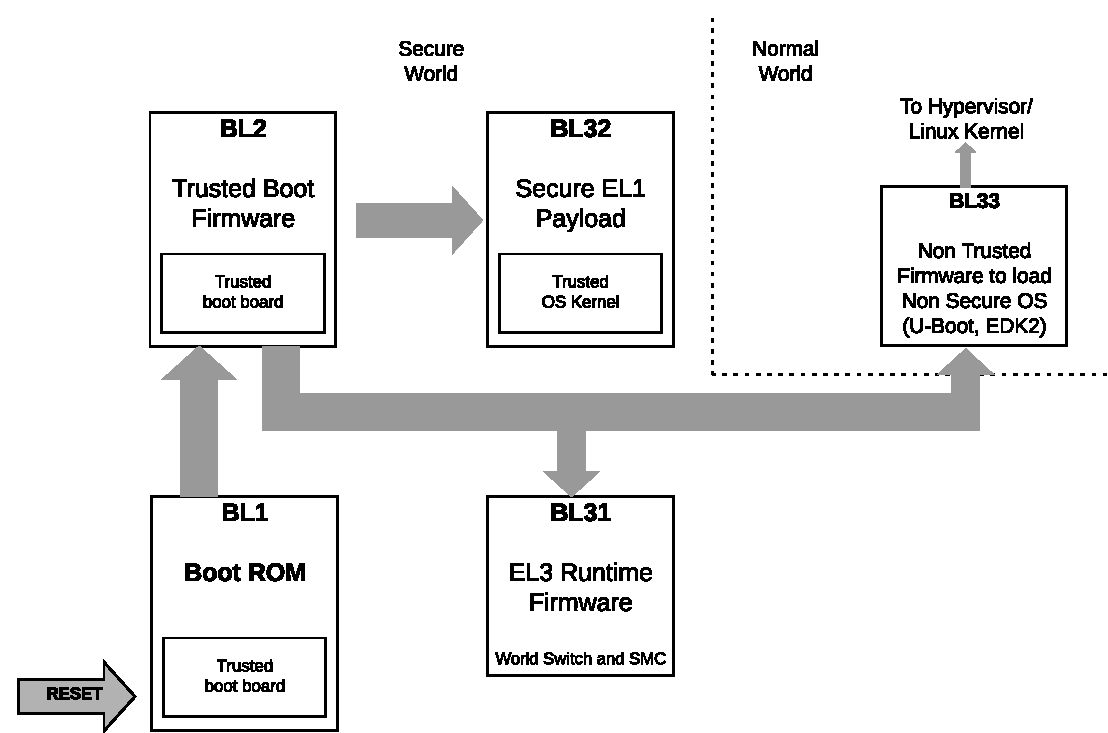
\includegraphics[width=\columnwidth]{fig/boot_process.pdf}  
\caption{ARM TrustZone Boot Sequence.}
\label{fig:bootsequence}
\end{figure}
%%%%%%%%%%%%%%%%%%%%	

%The first stage consists of two components: a platform dependent (e.g., HiKey) l-loader~\cite{lloader} 
%and the first stage of ATF boot (BL1). When the processor resets, it begins execution in Secure EL3 mode. 
%It jumps to a pre-set address in secure SRAM where a HiKey loader program (l-loader) redirects execution to 
%the ATF's first stage boot sequence. The first stage boot sequence sets up the EL3 runtime environment with
%the following sequence of actions:

%\begin{enumerate}
%\item  Initializes the exception vector table VBAR\_EL3
%\item  Initialize console and timer
%\item  Create EL3 MMU page table mappings for BL1 image
%\item  Load, verify and execute BL2 image in SRAM
%\end{enumerate}

%The second stage (BL2) sets up the EL1 runtime environment through a similar sequence of actions:

%\begin{enumerate}
%\item  Initializes the exception vector table VBAR\_EL1
%\item  Configure SRAM and CPU (e.g., clock rate, frequency dividers etc,.)
%\item  Create EL1 MMU page table mappings for BL2 image
%\item  Load, and verify BL31, BL32, Bl33 images in SRAM
%\end{enumerate} It (1)

%The third stage (BL3) is further divided into three sub-stages: BL31, BL32, and BL33.

%The first sub-stage (BL31) is the secure monitor. To execute at EL3, BL2 jumps to BL31 using an 
%\textit{smc} exception. Execution flow is redirected to the exception table pointed to by VBAR\_EL3, 
%which was set up during BL1. It is the last boot stage that executes in secure SRAM. It performs the 
%following sequence of actions:

%\begin{enumerate}
%\item  Re-initialize the exception vector table VBAR\_EL3 to a new runtime exception table
%\item  Initialize a \textit{cpu\_data\_t} structure per CPU to store pointers to the CPU's secure
% (\textit{opteed\_context\_t}) and non-secure contexts (\textit{cpu\_context\_t})
%\item  Allocate a C runtime stack for each CPU to use
%\item  Create EL3 MMU page table mappings for BL31 secure monitor image
%\item  Initialize the general interrupt controller (GIC), DMA, power control and real-time clock
%\item  Set up OP-TEE OS (EL1) entry-points and initialize secure CPU contexts
%\end{enumerate}

%The second sub-stage (BL32) contains the secure OP-TEE OS and runs at EL1 in the secure world. Currently, 
%ATF supports both OP-TEE OS and NVIDIA TLK~\cite{tlk}, although only OP-TEE OS seem to be actively 
%supported. The initialization procedure for the secure OS is rather complicated but involve the following 
%key steps:

%\begin{enumerate}
%\item Map a portion of unsecure DRAM (e.g., Hikey board -- 16MB) for OP-TEE OS
%\item Initialize each CPU with a secure context
%\item Re-initialize VBAR\_EL1 register to point to the same exception table pointed to by VBAR\_EL3
%\item Return a \textit{thread\_vector\_table} to the secure monitor that specifies entry-points 
%into OP-TEE OS
%\end{enumerate}

%The entry-points are stored by the secure monitor's handler (e.g., \textit{opteed\_smc\_handler}). 
%The handler operates as a state machine that controls all transitions between OP-TEE OS and normal world OS. 
%If the calling world is normal world, it performs the context switch to the secure world, and vice versa. 
%If also handles transitions due to RPC, interrupts and the initial boot process. The handler also initializes 
%and sets up the \textit{intr\_type\_desc}, which controls the interrupt routing model. The interrupt routing
%model specifies the destination world for IRQ and FIQ exceptions. The availability of these interrupts can be 
%masked by control bits in the SPSR registers.

%Once OP-TEE OS is initialized and returns to the secure monitor, the secure monitor then loads and boots 
%the normal world OS (Bl33). The third sub-stage (BL33) contains the normal world OS (Linux) and its 
%bootloader (EUFI/GRUB). This is the first stage that executes in the normal world. The boot sequence from 
%this point on is as-is for systems without TrustZone.

%Context switching between secure (BL32) and normal world (BL33) is handled by the secure monitor 
%(BL31). For each processor mode in~\ref{Tbl-TrustZone}, there are two stack pointers: one
%mode-specific stack pointer SP\_ELn and one general purpose stack pointer SP\_EL0. SP\_EL0 is 
%saved on context switches, while the mode-specific SP\_ELn is used to store the location of the 
%saved context. A context consists of all the EL3 and EL1 system registers,and all general purpose 
%registers (x0-x29, SP\_EL0, lr). The full list of relevant registers is defined with the
%\textit{DEFINE\_REG\_STRUCT} macro in the source code. When switching contexts, the secure monitor 
%controls the destination privilege level, interrupt masks and security state by modifying the NS-bit 
%in SCR and the interrupt mask and mode bits in SPSR.

\subsection{OP-TEE OS} 
 
\textbf{OP-TEE OS} is a small operating system that has been designed to run in the TrustZone backed TEE. It supports multi-threading and memory management, and some peripheral control over GPIO pins. Despite being a multi-threaded multi-core operating system, OP-TEE does not have a scheduler. OP-TEE does not differentiate between single core and multicore hardware - which core it runs on depends on which core was in use in the normal world user-space when the SMC call was initiated. On receiving the SMC call, the first trap occurs to the \textit{cpu\_on\_handler()} call on a fixed core (usually core 0), and it finishes with the SMC switching back to ARM-TF (EL3) and then the dispatcher does the world change to another core. 

Communication between the normal world and secure world occurs over buffers that are allocated by the normal world but are managed by the secure world. These buffers are used to pass information to and from the secure world for tasks such as TEE function invocation and Normal world filesystem access from within the TEE. 

OP-TEE OS provides APIs that can be used to construct user space trusted applications running in secure world (EL0 in secure world). OP-TEE OS applications conform to the GlobalPlatform Internal API~\cite{globalplatformAPI} where each trusted application must implement a set of well-defined functions as entry-points. These trusted applications run in the secure world user space (Secure EL0 in Table ~\ref{tab:privilege_levels}). Trusted applications can have a single-instance running in the secure world. Trusted Applications can, however, have multiple sessions active with the normal world. Client applications in the normal world invoke these trusted applications through a similar set of GlobalPlatform Client APIs. The flow of one such API call - to load a trusted application and establish a session with the trusted application is shown in Figure ~\ref{fig:ta_open}.

%%%%%%%%%%%%%%%%%%%%
\begin{figure}
\centering
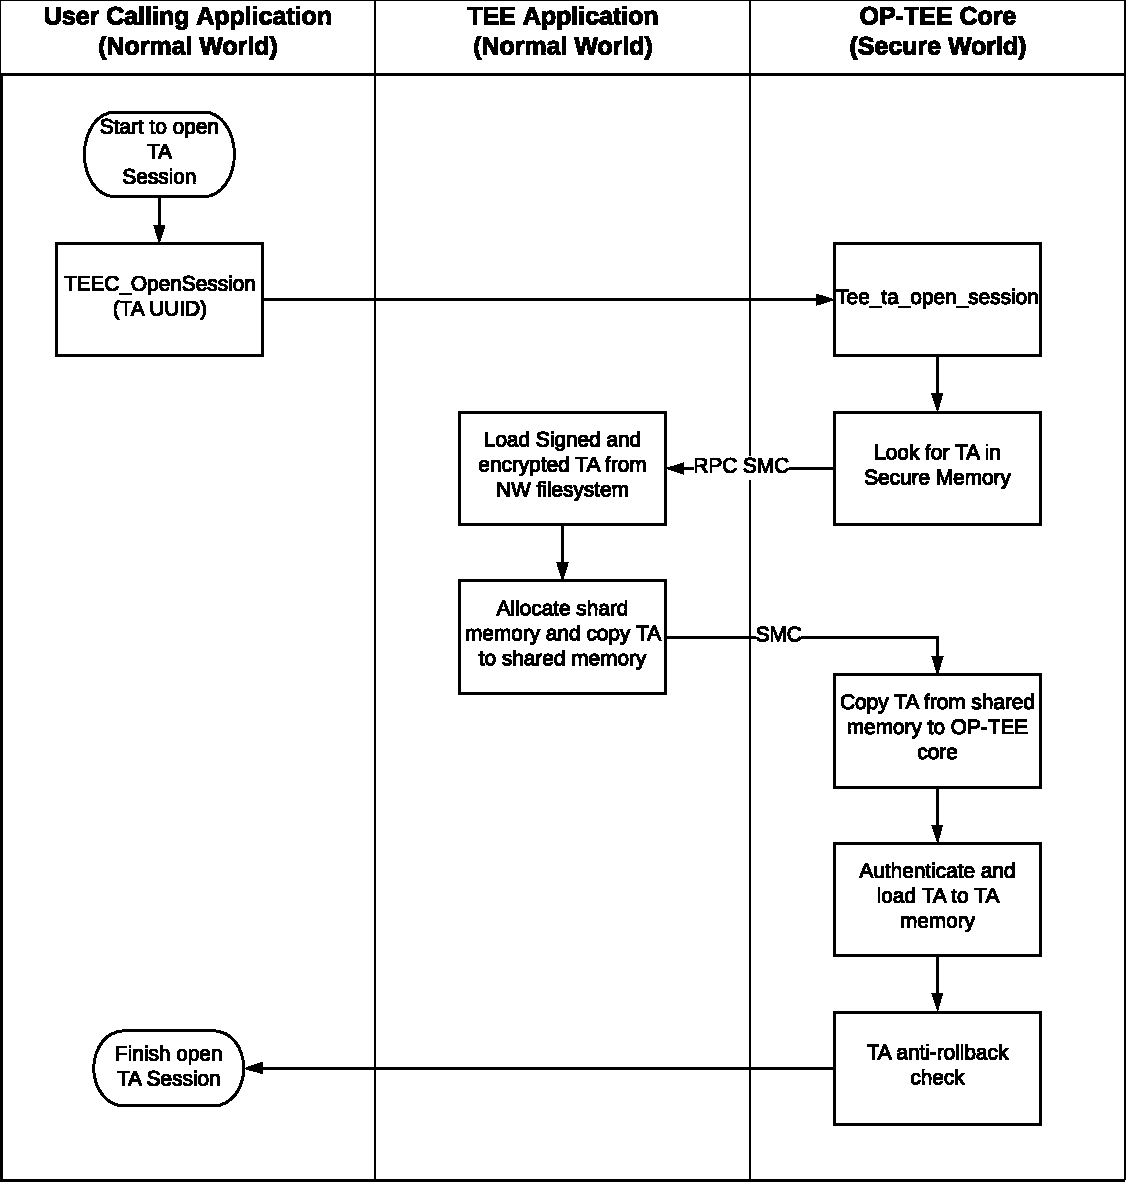
\includegraphics[width=\columnwidth]{fig/TA_Open.pdf}  
\caption{OP-TEE API calls to open A TA session}
\label{fig:ta_open}
\end{figure}
%%%%%%%%%%%%%%%%%%%%

% Client API~\cite{globalplatformAPI}. The list of functions are listed in 
% Table~\ref{Tbl-GlobalPlatformAPI}. We use these APIs and secure storage provided by OP-TEE OS to build 
% our multi-session trusted capsule application at the core of our trusted capsule monitor. Any call into 
% trusted applications from the normal world are serialized on the normal world side by the TrustZone 
% device driver.   

% %\begin{adjustwidth}{-0.75in}{-0.75in}
% %\noindent\makebox[\textwidth]{%
% \begin{table*}[t]
% \small
% \begin{center}
% \begin{tabular}{ |p{0.3\textwidth}|p{0.25\textwidth}|p{0.35\textwidth}| } 
%  \hline
%  \textbf{Internal API} & \textbf{Client API} & 
% \textbf{Function} \\\hline\hline 
%  CreateEntryPoint & InitializeContext & Initialize a context in TrustZone driver \\\hline
%  DestroyEntryPoint & FinalizeContext & Deletes a TrustZone context\\\hline
%  OpenSessionEntryPoint & OpenSession & Creates an instance of the 
% trusted application \\\hline
%  CloseSessionEntryPoint & CloseSession & Destroys an instance of the 
% trusted application \\\hline
%  InvokeCommandEntryPoint & InvokeCommand & Call one of trusted 
% application's functions \\\hline
%  - & RegisterSharedMemory & Registers a chunk of memory for use between 
% the two worlds\\\hline
%  - & AllocateSharedMemory & Allocate a chunk of memory from the shared 
% memory pool\\\hline
%  - & ReleaseSharedMemory & Free a chunk of memory allocated from the 
% shared memory pool\\\hline
%  - & RequestCancellation & Request an instance of trusted application to 
% stop and return\\\hline
% \end{tabular}
% \caption[Linaro OP-TEE API.]{Linaro OP-TEE API. Internal APIs are used by trusted applications 
% and are prefixed by \textit{TA\_}. Client APIs are used by the normal world and are prefixed 
% by \textit{TEEC\_}.} 
% \label{Tbl-GlobalPlatformAPI}
% \end{center}
% \end{table*}
% %}
% %\end{adjustwidth}

% \subsection{OP-TEE Linux Driver}

% \textbf{OP-TEE Linux Driver} provides the normal world OS (Linux) access to TrustZone. 
% It represents TrustZone as a device file, which can be accessed from the normal world through 
% the set of APIs listed in Table~\ref{Tbl-GlobalPlatformAPI} from both user and kernel space. 
% The TrustZone driver is responsible for two main tasks -- (1) calling into trusted applications 
% running in TrustZone and (2) handling RPC requests from OP-TEE OS (e.g., file system, shared memory 
% allocations). For trusted capsules, we extended the limited set of RPC calls available to the 
% OP-TEE OS to include networking and direct file system operations. The TrustZone driver executes 
% RPCs by using the OP-TEE Supplicant. 

% When the TrustZone driver calls into the secure world, it uses two unique identifiers -- "session 
% object" and "function ID". Each trusted application instance is represented by a "session" and each 
% function that the trusted application can perform by a "function ID". Together, these two identifiers 
% specify the entry point for the call into secure world. Function parameters are passed by value or by 
% reference through shared memory between the two worlds. 

% %Shared memory can either be allocated and re-used by the normal world application or it can be temporary, in 
% %which case the allocation and de-allocation occurs transparently. In both cases, moving data from client 
% %buffers require a copy to and from the shared memory between the two worlds. 

\subsection{OP-TEE Supplicant}

\textbf{OP-TEE Supplicant} takes RPC invocations from OP-TEE Linux Driver and executes the equivalent 
system calls through the normal world OS to access the relevant peripheral devices. These peripheral 
devices can include file system block devices and network cards for I/O. 
Linux \textit{dmabuf} and \textit{mmap} are used to pass data between the user space
OP-TEE supplicant and kernel space OP-TEE Linux Driver. 
Only a single instance of the OP-TEE supplicant 
can run at any given time and this is enforced by the Linux TEE driver.